\chapterimage{07_Sipanje.jpg} % Chapter heading image

\chapter{Sipanje}
V tem poglavju bomo na kratko predstavili sipanje svetlobe in z Rayleighovim
sipanjem na atomih in molekulah pojasnili modro barvo neba. Izpeljali bomo 
kotno odvisnost sipane svetlobe in njeno polarizacijo, poglavje pa zaključili
z opisom Miejevega sipanja.

\section{Sipanje in sipalni presek}
V petem poglavju smo podrobneje spoznali, kako se uklanja elektromagnetno 
valovanje, ki vpada na oviro. Uklonski integral, ki smo ga zapisali,
je dobro opisal pojave tako v bližnjem kot v daljnem polju. Kadar pa ovira,
na katero vpada elektromagnetno valovanje, ni ploščata in je 
po velikosti primerljiva z valovno dolžino svetlobe ali še manjša, je treba 
pojav obravnavati drugače. Čeprav gre formalno gledano za podoben pojav,
v tem primeru ne govorimo več o uklonu, ampak o sipanju svetlobe.

Sipanje svetlobe pomeni spremembo smeri vpadne svetlobe zaradi vpada na majhne delce. 
Majhni delci so lahko posamezni atomi, molekule, drobne kapljice ali kroglice, 
nepravilnosti v snovi, lokalne fluktuacije v gostoti snovi ... 
\begin{figure}[!h]
\centering
\includegraphics[width=7truecm]{slike/06_photo_soap.jpg}\hfill
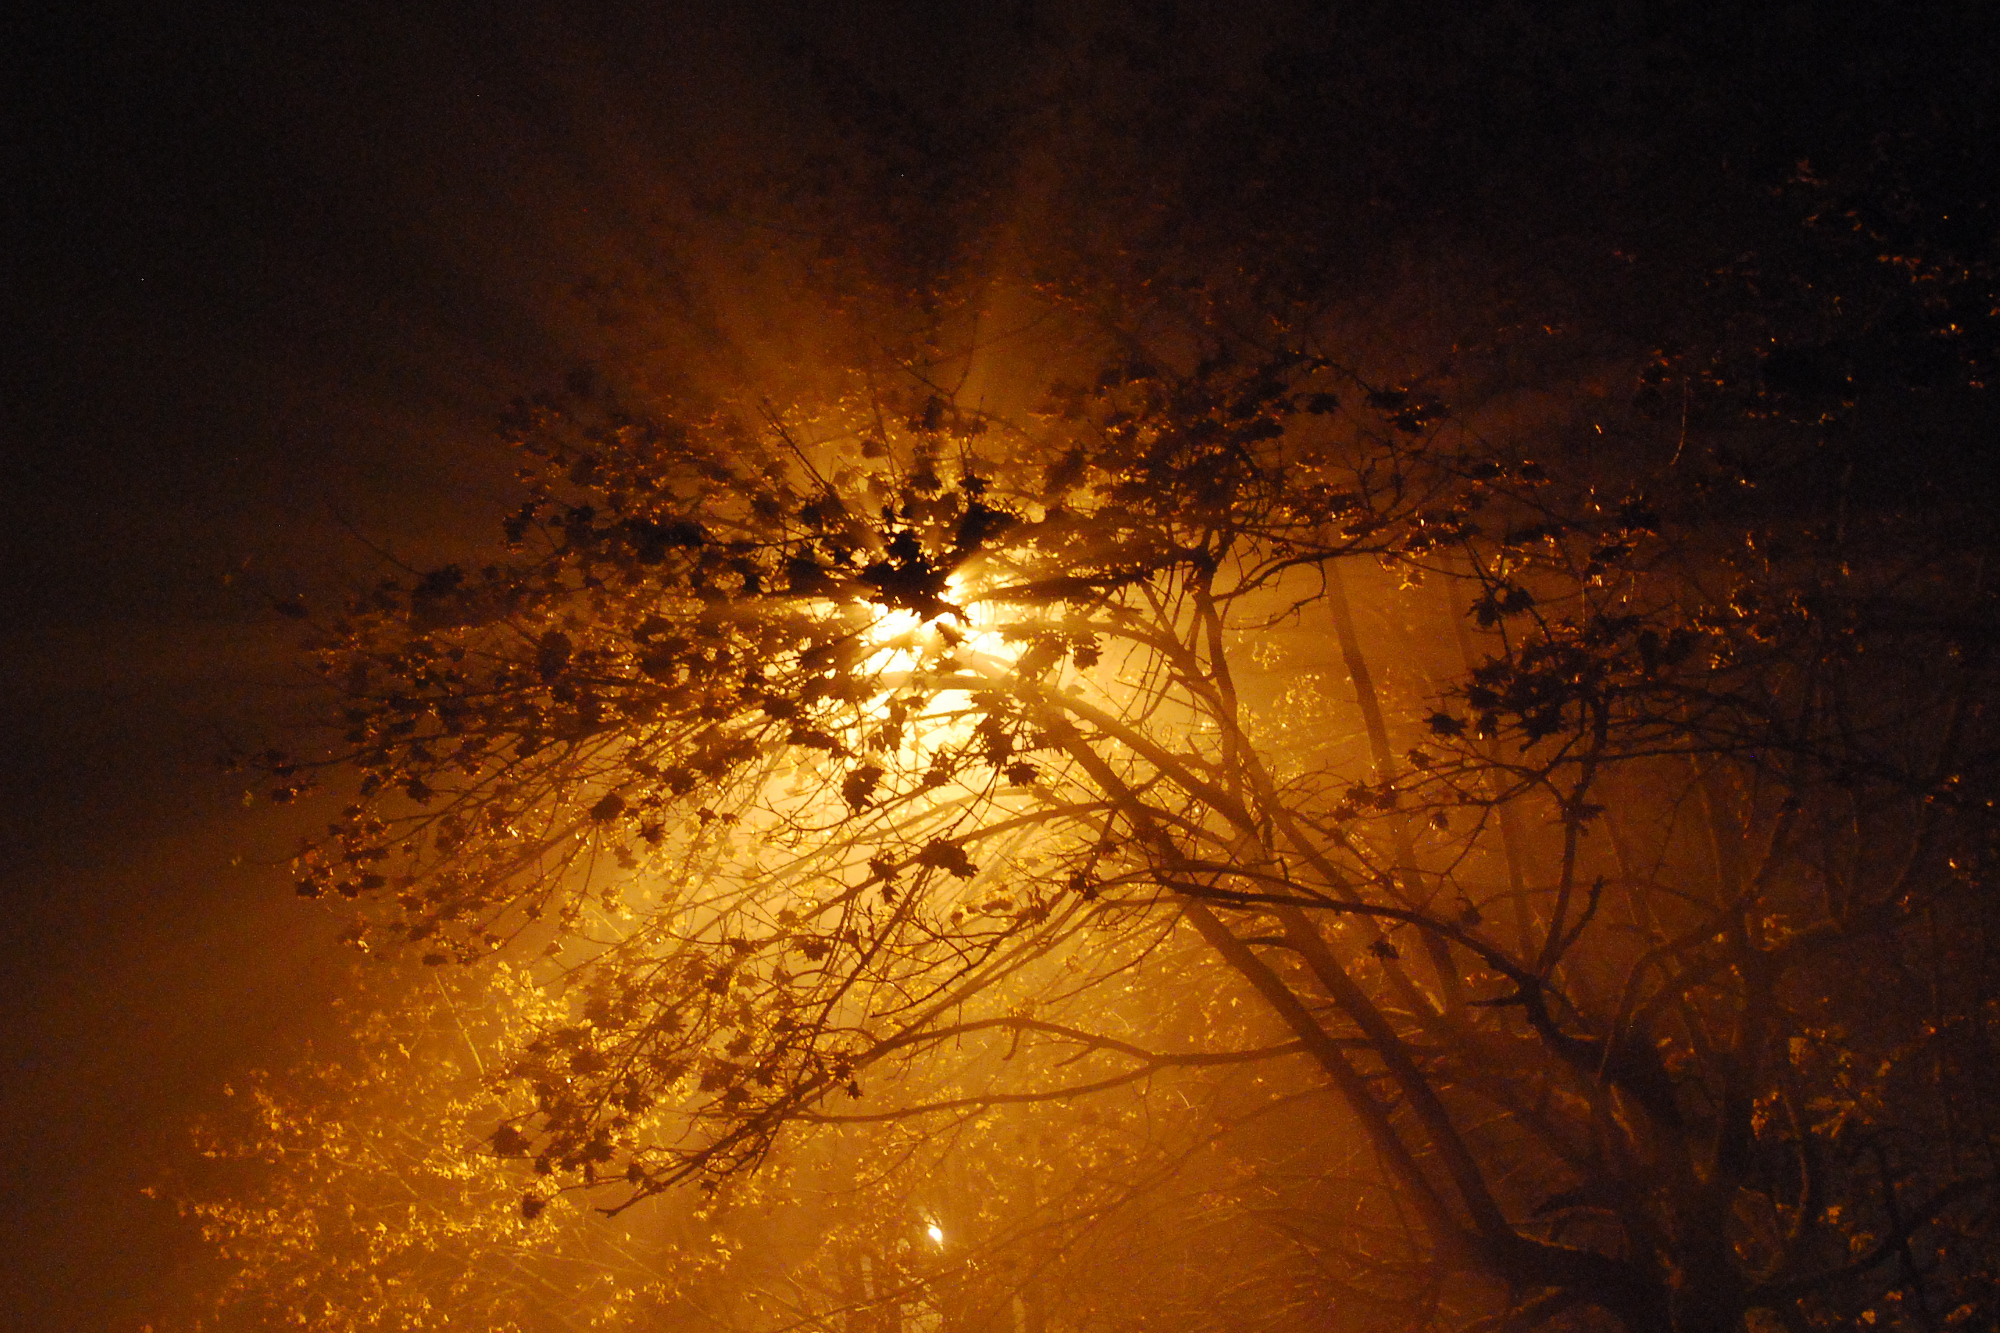
\includegraphics[width=7truecm]{slike/07_megla.jpg}
\caption{Sipanje svetlobe v mešanici vode in mleka (a) ter sipanje svetlobe 
cestne svetilke v megli (b). ZAMENJAJ FOTKO!!!}
\label{fig:07_Sipanje}
\end{figure}

V klasičnem Lorentzevu modelu atoma opišemo vezan elektron kot harmonski 
oscilator (razdelek~\ref{chap:lomni}). Ko na atom vpade
elektromagnetno valovanje, oscilirajoče električno polje deluje na elektron in 
ga periodično izmika iz ravnovesne lege. Nastali oscilirajoči električni dipol 
deluje kot antena in oddaja (seva) elektromagnetno valovanje. V velikih 
homogenih območjih se prispevki vseh atomov izpovprečijo in svetloba
se širi zgolj v vpadni smeri. Kadar pa je območje nehomogeno in se dielektrična
konstanta razlikuje znotraj območja, se prispevki posameznih atomov med seboj
razlikujejo. Posledično se svetloba širi tudi v smereh, ki 
se razlikujejo od vpadne smeri -- se siplje. Pri obravnavi se omejimo na 
vpadno valovanje, katerega frekvenca je daleč od resonančnih frekvenc atoma.
Takrat sta amplituda in frekvenca nihanja praktično neodvisni od frekvence 
vpadnega valovanja, vpadna svetloba pa se ne absorbira. 

Zaradi sipanja svetlobe se gostota svetlobnega toka v smeri vpadnega valovanja
zmanjšuje, kar imenujemo slabljenje, atenuacija ali ekstinkcija. Podobno učinkuje tudi 
absorpcija svetlobe v snovi, zato je celotno slabljenje sestavljeno iz dveh 
prispevkov: sipanja in absorpcije. Mi se bomo omejili zgolj na dielektrične 
snovi, ki svetlobe ne absorbirajo. Sipanje, pri katerem se svetloba ne absorbira
in energija ne izgublja, imenujemo elastično sipanje.

Naj svetloba z gostoto svetlobnega toka $j$ vpada na tanko plast snovi 
vzdolž smeri $z$. Prostornina osvetljenega dela naj bo $V = S \Delta z$,
v njem pa naj bo $N$ sipalcev, to je delcev, na katerih se svetloba siplje. 
Vsak od sipalcev prispeva k zmanjšanju svetlobnega toka:
\beq
\Delta P_1 = - \sigma_S j,
\label{eq:07_01}
\eeq
pri čemer smo vpeljali $\sigma_S$ kot sipalni presek. Sipalni presek delca ima sicer
enoto ploščine, vendar se razlikuje od prečnega preseka sipalnega delca. Lahko je 
precej večji od geometrijskega preseka delca, lahko pa tudi manjši od njega. Poleg
tega je sipalni presek odvisen od valovne dolžine elektromagnetnega valovanja, 
ki vpada na delec. Njegova velikost je določena s tem, kako močno vpliva na vpadno 
svetlobo: delci z večjim sipalnim presekom bolj sipljejo svetlobo in obratno, 
delci z manjšim sipalnim presekom manj zmotijo potek vpadnega valovanja.

Skupni prispevek vseh delcev v osvetljenem delu snovi k zmanjšanju svetlobnega toka
je potem:
\beq
\Delta P = - N \sigma_S j.
\label{eq:07_02}
\eeq
Vpeljemo gostoto sipalcev $\varrho = N/V$ in dobimo:
\beq
\Delta P = - \sigma_S j\,\varrho S \Delta z.
\label{eq:07_03}
\eeq
Izraz delimo s presekom snopa $S$ in ga zapišemo v diferencialni obliki:
\beq
dj = \frac{dP}{S} = - \sigma_S j\, \varrho dz
\label{eq:07_04}
\eeq
oziroma:
\beq
\frac{dj}{j} = - \sigma_S\, \varrho dz = -\mu dz.
\label{eq:07_05}
\eeq
Vpeljali smo $\mu$ kot koeficient slabljenja (tudi atenuacijski ali ekstinkcijski 
koeficient). Sorazmeren je gostoti delcev, na katerem se svetloba siplje, sorazmernostni
faktor pa je sipalni presek. Izraz integriramo in dobimo:
\boxeq{eq:BL}{
j(z) = j(z=0) e^{-\mu z}.
}
Zapisana enačba opisuje eksponentno pojemanje intenzitete vpadne svetlobe zaradi 
sipanja in je povsem analogna Beer-Lambertovem zakon za absorpcijo svetlobe v snovi. 

*** Dodaj foto. Recimo mleko in črnilo, v mleku sipanje, v črnilu absorpcija?***

\section{Rayleighovo sipanje}
Najprej si podrobneje oglejmo sipanje na delcih, ki so bistveno manjši 
od valovne dolžine svetlobe in za katere velja: $R \ll \lambda$ oziroma 
$kR \ll 1$, pri čemer je $R$ značilna dimenzija delca. Tako sipanje imenujemo 
Rayleighovo sipanje po angleškemu fiziku Lordu Rayleighu (1842--1919). 

Zaradi enostavnosti in nazornosti se omejimo na sipanje na 
kroglicah z dielektričnostjo $\varepsilon$. Svetloba naj se širi v smeri
$x$, njena polarizacija pa naj bo vzdolž osi $z$ (glej sliko~\ref{}).
Kadar je polmer kroglice bistveno manjši od
valovne dolžine vpadnega valovanja, lahko privzamemo, da je električno polje 
vpadnega valovanja znotraj celotnega delca enako. 
Ob vpadu svetlobe  se v delcu inducira polarizacija $\mathbf{P}$, ki je 
vzporedna vpadnemu polju $\mathbf{E}$. Iz zveze:
\beq
\mathbf{D} = \varepsilon \varepsilon_0 \mathbf{E} = \varepsilon_0 \mathbf{E} + \mathbf{P}
\label{eq:07_06}
\eeq
izrazimo polarizacijo kot:
\beq
\mathbf{P} = \varepsilon_0 (\varepsilon -1)\mathbf{E}.
\label{eq:07_07}
\eeq
Vpadno polje je oscilirajoče:
\beq
\mathbf{E} = \hat{\mathbf{e}}_z\, E(\mathbf{r}) e^{-i \omega t},
\label{eq:07_08}
\eeq
zato je oscilirajoča tudi inducirana polarizacija. Električni dipolni
moment dielektrične kroglice s polmerom $R$ je potem:
\beq
\mathbf{p} = \mathbf{P}\,V = \mathbf{P}\left(\frac{4\pi R^3}{3}\right) = 
\varepsilon_0 (\varepsilon -1)\left(\frac{4\pi R^3}{3}\right)\mathbf{E},
\label{eq:07_09}
\eeq
pri čemer smo upoštevali enačbo~(\ref{eq:07_07}). Vstavimo jakost električnega
polja (enačba~\ref{eq:07_08}) in dobimo:
\beq
\mathbf{p} = \mathbf{P}\,V = 
\varepsilon_0 (\varepsilon -1)\left(\frac{4\pi R^3}{3}\right)
\hat{\mathbf{e}}_z\, E(\mathbf{r}) e^{-i \omega t} = \mathbf{p}_0\,e^{-i \omega t}.
\label{eq:07_09a}
\eeq
S tem smo pokazali, da se v delcu, ko nanj vpada elektromagnetno valovanje, 
inducira oscilirajoči električni dipol. 

\begin{remark}
Zavedati se moramo, da zapisani izraz (enačba~\ref{eq:07_09a})
velja zgolj za delce v vakuumu, kjer je dielektričnost okolice delca enaka 
$\varepsilon_1=1$. Kadar pa je delec z dielektričnostjo $\varepsilon_2$ obdan 
s snovjo z dielektričnostjo $\varepsilon_1$, je treba upoštevati le razliko v polarizaciji
med delcem in okolico (presežno polarizacijo) $\Delta \mathbf{P}$. 
Enačbo~(\ref{eq:07_07}) na splošno zapišemo kot:
\beq
\Delta \mathbf{P} = \varepsilon_0 (\varepsilon_2 -\varepsilon_1) \mathbf{E} = 
\varepsilon_0 \Delta \varepsilon \mathbf{E},
\label{eq:07_10}
\eeq
kjer smo vpeljali $\Delta \varepsilon = \varepsilon_2 - \varepsilon_1$. 
Inducirani dipolni moment sipalca je potem:
\beq
\Delta \mathbf{p}= \Delta \mathbf{P}\,V = \Delta \varepsilon 
\left(\frac{4\pi R^3}{3}\right)\varepsilon_0 \hat{\mathbf{e}}_z\, E(\mathbf{r})
e^{-i \omega t}=\Delta \mathbf{p}_0\,e^{-i \omega t}.
\label{eq:07_11}
\eeq
Zapis je torej povsem podoben, le dielektrično konstanto je treba zapisati relativno 
glede na dielektričnost okolice.

Kadar sipalec ni en sam, ampak jih je več, je treba upoštevati tudi prispevke okoliških
delcev na inducirano polarizacijo v posameznem delcu. To naredimo z zapisom lokalnega polja, 
kot smo naredili v poglavju in člen $\Delta \varepsilon$ v izračunu za inducirano polarizacijo 
nadomestiti s členom:
\beq
\Delta \mathbf{p} \propto \left(\frac{3(\varepsilon-1)}{\varepsilon+2} \right)V \mathbf{E}_i,
\label{eq:07_22}
\eeq
pri čemer je $\varepsilon = \varepsilon_2/\varepsilon_1$. Ostalo se ne spremeni.
\end{remark}

Sinusno nihajoči električni dipol oddaja elektromagnetno valovanje -- seva. Sevalno 
polje v velikih oddaljenostih od dipola zapišemo 
kot:\footnote{Glej npr. Strnad, {\it Fizika, drugi del}, DMFA-založništvo (2018) in
Podgornik in Vilfan, {\it Elektromagnetno polje}, DMFA-založništvo (2012).}
\beq
\mathbf{E}_\mathrm{sev} = \frac{1}{4 \pi \varepsilon_0 c_0^2 r}
\left(\ddot{\mathbf{p}} \times \frac{\mathbf{r}}{r}\right)\times \frac{\mathbf{r}}{r}.
\label{eq:07_12}
\eeq
Vstavimo sinusno oscilirajoč električni dipol (enačba~\ref{eq:07_09a}) 
in izračunamo vektorski produkt. Dobimo:
\beq
\mathbf{E}_\mathrm{sev} = - \frac{\omega^2 p_0}{4 \pi \varepsilon_0 c_0^2}\sin 
\vartheta \left(\frac{e^{ikr - i\omega t}}{r}\right) \hat{\mathbf{e}}_\vartheta.
\label{eq:dipolE}
\eeq
V velikih oddaljenostih od dipola je jakost električnega polja vzdolž enotskega
vektorja $\hat{\mathbf{e}}_\vartheta$. V tem približku se amplituda polja, ki 
je odvisna tudi od polarnega kota $\vartheta$, zmanjšuje kot $1/r$.  

Podobno izračunamo tudi jakost magnetnega polja:
\beq
\mathbf{H}_\mathrm{sev} = \frac{1}{4 \pi  c_0 r}
\left(\ddot{\mathbf{p}} \times \frac{\mathbf{r}}{r}\right)\!\!,
\label{eq:07_13}
\eeq
od koder sledi: 
\beq
\mathbf{H}_\mathrm{sev} = - \frac{\omega^2 p_0}{4 \pi c_0}\sin \vartheta
\left(\frac{e^{ikr - i\omega t}}{r}\right) \hat{\mathbf{e}}_\varphi.
\label{eq:dipolH}
\eeq
Jakost magnetnega polja je pravokotna na smer dipola in hkrati tudi na smer
jakosti električnega polja. 

Gostoto energijskega toka sevalnega polja izračunamo kot povprečje 
Poyntingovega vektorja (enačba~\ref{eq:Poyntingov}):
\boxeq{eq:dipolj}{
\mathbf{j}_\mathrm{sev} = \langle \mathbf{E}_\mathrm{sev}
\times \mathbf{H}_\mathrm{sev}  \rangle 
= \frac{\omega^4 p_0^2 \sin^2 \vartheta}{32 \pi^2 \varepsilon_0 c_0^3 r^2}
\mathbf{e}_r.
}
Poglejmo rezultat podrobneje. Smer gostote svetlobnega toka je radialno navzven, 
kar po meni, da se zaradi sevanja vpadni energijski tok preusmeri iz vpadne smeri
v druge smeri. Posledično amplituda v vpadni smeri slabi, v ostalih smereh pa se 
pojavi sipana svetloba. Amplituda gostote svetlobnega toka 
pojema obratno s kvadratom oddaljenosti od izhodišča, kar je v skladu
z ohranitvijo energije. Vidimo, da je sevalno polje odvisno od kota $\vartheta$,
to je kotom med smerjo polarizacije vpadne svetlobe in smerjo opazovanja. Vzdolž
smeri vpadne polarizacije sevanja ni, največje pa je v smeri pravokotno glede
na vpadno svetlobo.

Poleg kotne odvisnosti je zelo pomembna tudi sorazmernost gostote energijskega toka
od četrte potence frekvence vpadne svetlobe:
\boxeq{eq:rayleigh}{
\mathbf{j}_\mathrm{sev} \propto \omega^4 \propto \frac{1}{\lambda^4}.
}
Valovanja s krajšimi valovnimi dolžinami se tako bistveno bolj sipljejo kot valovanja 
z daljšimi valovnimi dolžinami. Povedano drugače: modra svetloba se siplje bistveno 
bolj od rdeče svetlobe. To ima zelo pomembno -- in vidno -- posledico.

Ponovimo, da to za primer, ko p0 ni odvisen od frekvence vpadnega valovanja. ! V modelu je 
lahko tudi v drugo smer odvisen - thomsonovo sipanje/blinc/poberaj.

\begin{example}{\bf Zakaj je nebo modro?}
Svetloba, ki s Sonca vpada na Zemljino površje, najprej prepotuje Zemljino atmosfero.
Pri tem se del svetlobe se absorbira (najizrazitejše so absorpcije v ultravijoličnem delu 
spektra na ozonski plasti ter na infrardečem spektru na molekulah vode in ogljikovega 
dioksida). Preostala svetloba potuje skozi atmosfero in se pri tem na molekulah v zraku
Rayleighovo siplje. Zaradi močne odvisnosti intenzitete sipanja od valovne dolžine svetlobe 
(enačba~\ref{eq:rayleigh}) se modri odtenki s krajšo valovno dolžino sipljejo bistveno bolj 
kot svetloba rdečih odtenkov z daljšo valovno dolžino. Na primer: svetloba z 
$\lambda = 400~\si{\nm}$ se siplje 16-krat močneje kot svetloba z $\lambda = 800~\si{\nm}$.
Ko opazujemo nebo, zaznavamo svetlobo, ki se na atmosferi siplje. Ker se modri odtenki sipljejo
bolj kot rdeči, vidimo nebo modro. 

Seveda se vprašamo, zakaj ne vidimo neba vijoličnega, saj 
ima vijolična svetloba še krajšo valovno dolžino in se zato še močneje siplje. Upoštevati 
moramo spekter sončeve svetlobe, v katerem je vijolična barva manj zastopana od modre, poleg
tega k temu prispeva tudi občutljivost očesa, ki se pri krajših valovnih dolžinah znatno 
zmanjša in vijolične barve ne zaznava tako močno kot modre. 

Na Luni, kjer ni atmosfere, je nebo povsem črno.
\end{example}

\begin{example}{\bf In zakaj je sončni zahod rdeč?}
Tudi rdeči sončni vzhodi in zahodi so posledica sipanja svetlobe na atmosferi. Takrat Sonce
leži nizko nad obzorjem in pot sončne svetlobe skozi atmosfero je razmeroma dolga.
Modra svetloba se močno siplje na vse strani, rdeča svetloba pa razmeroma malo. Večina
svetlobe, ki pride do opazovalca, je tako rdečkaste barve.
\end{example}

\begin{example}{\bf Sipanje nepolarizirane svetlobe.}
Naj bo sipalni delec vzdolž smeri $x$ vpada nepolarizirana svetloba. Električno
polje vpadne svetlobe razdelimo na dva prispevka: polarizacijo vzdolž osi $y$ in 
polarizacijo vzdolž osi $z$. Sipano svetlobo opazujemo v ravnini $xy$, v kateri
ležita valovni vektor vpadne svetlobe $\mathbf{k}_i$ in valovni vektor sipane svetlobe
$\mathbf{k}_s$. Kot med njima $\beta$ imenujemo sipalni kot.

Za del svetlobe, ki je polariziran v smeri $z$, se detektor nahaja 
v ekvatorialni ravnini ($\vartheta = 90\si{\degree}$) in 
$j_{\mathrm{sev}, z}$ je neodvisen od sipalnega kota $\beta$. Gostota energijskega
toka sipane svetlobe za del svetlobe, ki je polariziran vzdolž smeri $y$, pa je od kota
odvisna. Zapišemo zvezo $\vartheta = \pi/2+\beta$ in to upoštevamo pri zapisu sevalnega polja.
Skupno sipano polje je sestavljeno iz obeh prispevkov:
\beq
j_\mathrm{sip} = j_{\mathrm{sev}, y} + j_{\mathrm{sev}, z} = 
j_{\mathrm{sev}, 0}\sin^2\left(\pi/2+\beta \right) + 
j_{\mathrm{sev}, 0} = j_{\mathrm{sev}, 0}\left(1 + \cos^2\beta\right).
\label{eq:07_13}
\eeq
Kadar torej vpada nepolarizirana vpadna svetloba, je sipane svetlobe v smeri pravokotno 
na izvor dvakrat manj kot sipane svetlobe vzdolž vpadne smeri. Enako kot sipanja v smeri
naprej je tudi sipanja v smeri nazaj.
\end{example}

\begin{example}{\bf Polarizacija sipane svetlobe.}
Spoznali, smo, da je zaradi sipanja svetlobe nebo čez dan videti modro. Poglejmo še 
polarizacijo te modre svetlobe, če svetlobo opazujemo v smeri pravokotno glede na Sonce (glej 
sliko). Svetloba s Sonca je nepolarizirana. Komponenta svetlobe, 
ki je polarizirana pravokotno na Zemljino površje, v smeri opazovalca ne seva, polarizacija,
ki leži tangentno na Zemljino površje, pa seva. Svetloba, ki jo tako zazna opazovalec
na Zemlji, je polarizirana v smeri pravokotno na smer Sonca. V naravi polarizacija ni popolna,
saj prihaja do večkratnega sipanja, do sipanja na drugih, večjih delcih v atmosferi, za katere
Rayleighov približek ne velja, ipd. 
\end{example}

Vrnimo se k izrazu za gostoto energijskega toka sipane svetlobe (enačba~\ref{eq:dipolj})
in vanj vstavimo velikost induciranega dipolnega momenta (enačba~\ref{eq:07_11}). Na danem
mestu je gostota svetlobnega toka sipane svetlobe sorazmerna:
\beq
\mathbf{j}_\mathrm{sev} \propto \omega^4 p_0^2 \propto \frac{E^2V^2}{\lambda^4} 
\propto \frac{E^2 R^6}{\lambda^4}.
\label{eq:07_17}
\eeq
Razmerje med sipanim svetlobnim tokom in vpadno gostoto svetlobnega toka določa sipalni presek. Iz
zapisanega sledi, da je sipalni presek sorazmeren s šesto potenco polmera delca in obratno
sorazmeren s četrto potenco valovne dolžine svetlobe. 

Vpeljemo še sipalni izkoristek $Q_S$ kot razmerje med sipalnim presekom $\sigma$ in 
dejanskim prečnim presekom delca $S$. Zapišemo:
\beq
Q_S = \frac{\sigma}{S} \propto \frac{R^6}{\lambda^4 (\pi R^2)}\propto\left(\frac{R}{\lambda}\right)^4\!\!.
\label{eq:07_17}
\eeq
Četrta potenca odvisnosti sipalnega izkoristka od velikosti delcev je značilna za Rayleighovo sipanje.


\begin{example}{\bf Tyndallov pojav.}
Odvisnost  
 
\end{example}

\subsection*{Sipalna matrika}
Tudi pri sipanju navadno uvedemo matrični zapis. Vsako vpadno polarizacijo lahko obravnavamo, tako
da jo razstavimo na dve komponenti: eno, ki je vzporedna s sipalno ravnino $E_\parallel$, in drugo, ki 
je nanjo pravokotna $E_\perp$. V našem zapisu je tako $E_\parallel \parallel H$ in
$E_\perp \parallel V$. 
\beq
\mathbf{E}_s = 
\left[\begin{array}{c}
E_{s,H}\\
E_{s,V}\\
\end{array}\right]
= \left[\begin{array}{c}
E_{s, \parallel}(\beta)\\
E_{s, \perp}(\beta)\\
\end{array}\right] = 
\left[\begin{array}{cc}
S_2 & S_3 \\
S_4 & S_1\\
\end{array}\right] 
\left[\begin{array}{c}
E_{i, \parallel}(\beta)\\
E_{i, \perp}(\beta)\\
\end{array}\right] 
\left(
\frac{e^{ik(r-x)}}{ikr}
\right)\!\!.
\label{eq:07_14}
\eeq
Pri tem je matrika amplitudna sipalna matrika, ki je na splošno funkcija zenitalnega
in azimutalnega kota (če delec ni povsem okrogel), ki poruši simetrijo. Vektor v zgornjem
zapisu predstavlja optično polje vpadne svetlobe, zadnji člen pa je transportni faktor,
ki je odvisen od razdalje med sipalcem in detektorjem $r$, ter od globine, v kateri
je prišlo so sipanja (z).

V praksi navadno merimo gostoto energijskega toka sipane svetlobe:
\beq
j_s \propto |E_{s, \parallel}|^2 + |E_{s, \perp}|^2.
\label{eq:07_15}
\eeq
Ker sta polarizaciji ortogonalni, mešani členi ničesar ne prispevajo. Potem sipalno matriko
za gostoto svetlobnega toka zapišemo kot:
\beq
\left[\begin{array}{c}
j_{s, \parallel}(\beta)\\
j_{s, \perp}(\beta)\\
\end{array}\right] = 
\left[\begin{array}{cc}
|S_2|^2& 0\\
0 & |S_1|^2\\
\end{array}\right] 
\left[\begin{array}{c}
j_{i, \parallel}(\beta)\\
j_{i, \perp}(\beta)\\
\end{array}\right]\!\!.
\label{eq:07_16}
\eeq

.. Kakšen komentar, zakaj je to dobro, primer? .. Zakaj so indeksi tako čudno?

\section{Miejevo sipanje}
Sipanje svetlobe na delcih, ki so po velikosti primerljivi z valovno dolžino vpadne svetlobe, imenujemo
Miejevo sipanje po nemškem fiziku Gustavu Mieju (1868--1957). Kadar je polmer delcev $R\approx \lambda$
ali večji, približek sipalca kot točkastega dipola ni ustrezen. V tem primeru se moramo lotiti problema
bolj natančno, tako da z reševanjem Maxwellovih enačb izračunamo polje znotraj in zunaj delca ter
ustrezno upoštevamo robne pogoje med delcem in okolico. Če je delec okrogel, iščemo rešitve v sferičnih 
koordinatah. Pojav dovolj dobro opišemo, če rešujemo skalarno Helmholtzevo enačbo (enačba..) in rešitve
poiščemo z metodo separacije spremeljivk:
\beq
E_{lm}(r,\vartheta, \varphi) = R_l(r) \Theta_l^m(\vartheta) \Phi_m(\varphi) = 
E_0 e^{im\varphi}P_l^m (\cos \vartheta) Z_l (kr).
\label{eq:07_20}
\eeq
Pri tem $P$ označujejo pridružene Legendrove polinome, $Z$ pa sferične Besslove funkcije prvega
ali drugega reda. Celotno sipano polje zapišemo kot vsoto vseh prispevkov:
\beq
E = \sum_{l,m} A_{l,m}E_{l,m}.
\label{eq:07_21}
\eeq
Navedene funkcije (vektorski sferični harmoniki) tvorijo poln ortogonalni sistem stanj. V sferične
harmonike zato lahko razvijemo tudi vpadno valovanje. Celotno polje v prostoru potem zapišemo
kot superpozicijo vpadnega in sipanega valovanja. Koeficiente $A$ pred različnimi členi pa dobimo
iz robnih pogojev. 

Z računom ugotovimo, da - podobno kot pri Fabry-Perotovem interferometru - tudi v sferičnih delcih
lahko pride do resonance, kadar sta polmer delca in valovna dolžina v ustreznem razmerju. Takrat 
je sipano polje oziroma energijski tok sipanega valovanja še posebej šibek (ali velik). Po drugi
strani  pa sipalni izkoristek ni več tako izrazito odvisen od razmerja $R/\lambda$. GRAF. 

Tudi kotna odvisnosti $j(\beta)$ kaže številne minimume in maksimume. Prevladuje sipanje naprej (skica).


- beli oblaki.

- Zakaj so oddaljene gore bolj svetle /in modre/ od bližnjih?

- detektor megle/plina. manj svetlobe pride do detektorja.

***
Dodaj: 
Debye ali Miejevo sipanje - elastično na delcih ali molekulah, ki so primerljive
z valovno dolžino sverlobe, izrazito enenakomerno sipanje. Ni zelo odvisno od
valovne dolžine, kapljice v zraku - bel oblak in megla. 

Brillouinovo sipanje - neelastično, na trdni snovi, vzbudimo fonone, majhni premiki.

Ramanovo sipanje - neelastično, razlika v frekvencah je razlika v energijskih 
nivojih atomov in molekul. Zelo uporabno za analizo materialov, kemijsko sestavo.
Stokes, anti-stokes. 

Thompsonovo sipanje na nabitih delcih? Xray?

Uporaba sipanja, Rayleigh... Raman... 
